\documentclass{article}
\usepackage{amssymb}
\usepackage[utf8]{inputenc}
\usepackage{amsmath}
\usepackage[spanish]{babel}
\usepackage{tikz}
\usepackage{graphicx}
\newcommand{\N}{\mathbb{N}}
\newcommand{\R}[1]{$\mathbb{R}^#1$}
\newcommand{\Phisub}[1]{$\varphi_#1$}
\newcommand{\matriz}[4]{\begin{pmatrix}
#1 & #2\\
#3 & #4
\end{pmatrix}}


\providecommand{\norm}[1]{\lVert#1\rVert}
\usepackage{amsthm}
\usepackage{graphicx}

\newtheorem{definition}{Definición}[section]
\newtheorem{observation}{Observación}[section]
\newtheorem{theorem}{Teorema}[section]
\newtheorem{proposition}{Proposición}[section]
\newtheorem{lemma}{Lema}[section]
\newtheorem{corollary}{Corolario}[section]
\newtheorem{example}{Ejemplo}[section]
\newtheorem{exercise}{Ejercicio}[section]



\title{	

	\normalfont\normalsize
	\textsc{Universidad de Murcia}\\ 
	\vspace{25pt} % Whitespace
	\rule{\linewidth}{0.5pt} % Thin top horizontal rule
	\vspace{20pt}\\ % Whitespace
	{\huge FVVII: Tarea 1
}\\ % The assignment title
	\vspace{12pt} % Whitespace
	\rule{\linewidth}{2pt}\\ % Thick bottom horizontal rule
	\vspace{12pt} % Whitespace
	% 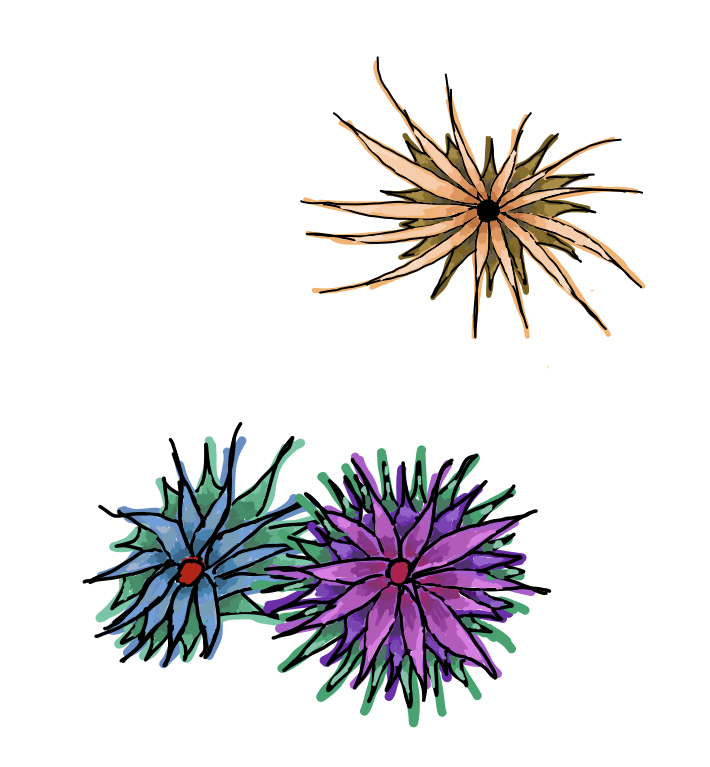
\includegraphics[scale=0.25]{floresportada.png}
}


\author{\LARGE Alonso Oma Alonso} % Your name

  
 
\date{\normalsize\today} % Today's date (\today) or a custom date



\begin{document}

\begin{titlepage}
	\maketitle
\end{titlepage}

\newpage
\tableofcontents
\newpage

\begin{section}{Problema}
	Sea $\mathcal{X}$ un conjunto, $\mathcal{A}  \subset P(\mathcal{X})$ una familia de subconjuntos de $X
$, e $Y \subset \mathcal{X}$. Denotemos $\mathcal{A}_y = \{A \cap Y: A \in \mathcal{A}\}$. Probar que las operaciones de generación e inducción se pueden intercambiar, es decir, $\sigma(\mathcal{A})_y = \sigma(\mathcal{A}_y)$.

\begin{definition}
	Sea $S \subset P(\mathcal{X})$. La intersección de todas las $\sigma$-álgebras que contienen a $S$ se denomina $\sigma$-ágebra generada por $S$ y se denota por $\mathcal{M}_S$.
\end{definition}

\begin{definition}
	Sea $\{\mathcal{X, \mathcal{M}}\}$ un espacio medible, y sea $A\in \mathcal{M}$. La $\sigma$-álgebra $\{A\cap B: B\in \mathcal{M}\}$ se denomina 
	$\sigma$-álgebra inducida en $A$ y se denota $\mathcal{M}_A$.
\end{definition}

La $\sigma$-álgebra generada por $\mathcal{A}\subset P(\mathcal{X})$ es la intersección de todas las $\sigma$-álgebras 
que contienen a $\mathcal{A}$. Es decir, $\sigma(\mathcal{A})$ es la menor $\sigma$-álgebra que contiene a $\mathcal{A}$ y, 
además, da lugar a un espacio medible. Por lo tanto, ahora podemos aplicar la definición de $\sigma$-álgebra inducida en el 
espacio $\{\mathcal{X}, \mathcal{M}_{\mathcal{A}}\}$. Entonces $\sigma(\mathcal{A})_y = \{Y\cap B: B \in \mathcal{M}\}$ será 
la $\sigma$-álgebra inducida en $Y$, y la denotaremos como $\mathcal{M}_{\mathcal{A}_y}$.

Ahora, veamos qué es $\sigma(\mathcal{A}_y)$: Por hipótesis, tenemos que $\mathcal{A}_y = \{A \cap Y: A \in \mathcal{A}\}$
la cuál no podemos dar por supuesto que es una $\sigma$-álgebra ya que no sabemos si $\{\mathcal{X}, \mathcal{A}\}$ es un 
espacio medible. Sin embargo, $\sigma(\mathcal{A}_y)$ sí que es una $\sigma$-álgebra, y además es la menor $\sigma$-álgebra 
que contiene a $\mathcal{A}_y$, por lo que la denominaremos $\mathcal{M'}_{\mathcal{A}_y}$.

\begin{itemize}
	\item Para ver que $\mathcal{M'}_{\mathcal{A}_y} \subset \mathcal{M}_{\mathcal{A}_y}$ vamos a ver que $\mathcal{A}_y \subset \mathcal{M}_{\mathcal{A}_y}$.
	Para ello es fácil ver que $\mathcal{A} \subset \mathcal{M}_{\mathcal{A}} \Longrightarrow \{Y \cap A: A \in \mathcal{A}\} \subset \{Y \cap B: B \subset \mathcal{M}_{\mathcal{A}}\}$.
	Pero como por definición $\mathcal{M'}_{\mathcal{A}_y}$ es la intersección de todas las $sigma$-álgebras que contienen a $\mathcal{A}_y$, entonces $\mathcal{M'}_{\mathcal{A}_y} \subset \mathcal{M}_{\mathcal{A}_y}$.

	\item Veamos ahora que $\mathcal{M}_{\mathcal{A}_y} \subset \mathcal{M'}_{\mathcal{A}_y}$: Esta la resolveremos por reducción al absurdo. Supongamos
	que no fuese cierto. Entonces existiría 

\end{itemize}


\end{section}

\end{document}
